\documentclass[]{article}

%funny text
\usepackage[utf8]{inputenc} % set input encoding (not needed with XeLaTeX)
\usepackage[T1]{fontenc}
\DeclareUnicodeCharacter{00A0}{ }

%packages
\usepackage[english]{babel}
\usepackage[nottoc,notlof,notlot]{tocbibind} % Put the bibliography in the ToC
\usepackage{hyperref} % use hyperlinked ToC
\usepackage{parskip}
\usepackage{booktabs} % for much better looking tables
\usepackage{array} % for better arrays (eg matrices) in maths
\usepackage{paralist} % very flexible & customisable lists (eg. enumerate/itemize, etc.)
\usepackage{verbatim} % adds environment for commenting out blocks of text & for better verbatim
\usepackage{subfig} % make it possible to include more than one captioned figure/table in a single float
\usepackage{listings} %for code listings
\usepackage{color} %for colored syntax highligting
\usepackage{rotating}
\usepackage{pdflscape}
\usepackage[]{algorithm2e}
\usepackage{multirow}
\usepackage{float}
\usepackage{mathtools}
\usepackage{amssymb}
\usepackage{geometry} % to change the page dimensions
\usepackage{indentfirst}
\usepackage[printonlyused]{acronym}
\usepackage[backend=bibtex, bibencoding=utf8]{biblatex}

\DeclarePairedDelimiter\ceil{\lceil}{\rceil}
\DeclarePairedDelimiter\floor{\lfloor}{\rfloor}

\graphicspath{ {assets/} }

\bibliography{biblib} 

%%% Page geometry
\geometry{a4paper} % or letterpaper (US) or a5paper or....
\geometry{margin=2.7cm}

%%% Paragraphs and text 
\setlength{\parindent}{4em}
\setlength{\parskip}{1em} 
\renewcommand{\baselinestretch}{1.3}
\setlength{\parskip}{10pt plus 1pt minus 1pt}

%%% Code listing
\definecolor{mygreen}{rgb}{0,0.6,0}
\definecolor{mygray}{rgb}{0.5,0.5,0.5}
\definecolor{mymauve}{rgb}{0.58,0,0.82}
\lstset{
basicstyle=\footnotesize\ttfamily,
commentstyle=\color{mygreen},
keywordstyle=\color{blue},
numberstyle=\tiny\color{mygray},
numbers=left,
tabsize=2,
frame=tb,
aboveskip=3mm,
belowskip=3mm,
breaklines=true,
breakatwhitespace=true,
showstringspaces=false,
columns=flexible
}
% to include a file as a listing: \lstinputlisting{intio.c}
% inline listing: \begin{lstlisting}[frame=single]

\hypersetup{colorlinks=true, linkcolor=black, citecolor=black, filecolor=black, urlcolor=black}

%%%%%%%%%%%%%%%%%%%%%%%%%%%%%%%%%%%%%%%%%%%%%%%%%
%%%%%%%%%%%%%%%%%%%%%%%%%%%%%%%%%%%%%%%%%%%%%%%%%

\title{A Wireless  Low Energy Ambulatory Electroencephalogram}
\author{Thomas Alexander Morrison (tm1810)}
\begin{document}



\begin{titlepage}
% \newgeometry{top=25mm,bottom=25mm,left=38mm,right=32mm}
\setlength{\parindent}{0pt}
\setlength{\parskip}{0pt}
% \fontfamily{phv}\selectfont

{
\Large
\raggedright
Imperial College London\\[17pt]
Department of Electrical and Electronic Engineering\\[17pt]
Final Year Project Report 2014\\[17pt]

}
\rule{\columnwidth}{3pt}

\vfill

\centering
% \includegraphics[width=0.7\columnwidth,height=60mm,keepaspectratio]{imgs/MyRobot.jpg}

\vfill

\setlength{\tabcolsep}{0pt}
\begin{tabular}{p{40mm}p{\dimexpr\columnwidth-40mm}}
Project Title: & \textbf{A Wireless  Low Energy Ambulatory Electroencephalogram} \\[12pt]
Student: & \textbf{Thomas Alexander Morrison} \\[12pt]
CID: & \textbf{00642176} \\[12pt]
Course: & \textbf{ISE4} \\[12pt]
Project Supervisor: & \textbf{James Mardell} \\[12pt]
Second Marker: & \textbf{Dr. Pants Georgiou} \\
\end{tabular}
\end{titlepage}

\clearpage





\clearpage

\section*{Abstract}
Certain neurological medical disorders require continuous monitoring to fully understand and diagnose. Examples of medical interest include epilepsy, syncope, multiple sclerosis, migraines, strokes, Parkinson’s and Alzheimer’s disease. \ac{EEG} is the recording of electrical activity along the scale, resulting from ionic current flows within the neurons of the brain and is useful for both diagnostic and monitoring such aforementioned conditions. Monitoring brain activity can help physicians understand certain characteristics, triggers, and the severity of the disorder. It may be possible to gauge the regions of the brain where the condition is originating and if the patient is a suitable candidate for treatment. 

However, symptoms from neurological disorders often appear sporadically and with little to no warning. Seizures vary from minutes to years apart, and sometimes are not realised or detected without proper equipment. Hospitalising patients for long periods of time is a costly option, and in such circumstances the patient could remain in hospital indefinitely.  Such circumstances lend themselves to an ambulatory system, where an outpatient can be monitored continuously without discomfort or hospitalisation, improving quality of life while decreasing costs. 

With the emergence of low power wireless technologies coupled with portable devices such as tablets and phones, it is a natural technological step to bring care and monitoring out of the hospital and into the home. Through leveraging low energy radio capable platforms, i.e. smartphones and tablets, in the context of an ambulatory EEG, it is possible to empower the patient to inexpensively take health care into their own home and out of the hospital. This project looks at maximising transmission of \ac{EEG} signals over the emerging wireless technology, \ac{BLE}. Further, while this project is targeted at EEG signals, there is no reason why this research and technology cannot be applied to other signals and systems, examples including glucose monitoring, electrocardiography and spirometers.

\cite{Blanco95}
\clearpage
\tableofcontents
\clearpage

%Don't be gay
\section{Acknowledgements}
The opporunity is taken here to express gratitude to all those who have directly contributed towards the project. 

Firstly, the project surperivsors, James Mardell, Chen Guangwei and Esther Rodriguez-Villegas for their. 

Cambridge Silicon Radio providing hardware and technical support. Employees particurarly are Adam Hill, Martin Spikings, Mark Wade, Neil Stewart and Simon. The recently launched uEnergy forum is an excellent source of . CSR also await a report on the speed of 

Guan from NYC

Other CSR1010 IC student

Dr. Nissim Zur, CEO of Vitelix Limited is an expert in low power wireless technologies, and has conversed over many aspects of the final chip used. Further, has also taken an interest in this project's work in regards to maximising the speed, and has requested the results be shared with him.

Finally, and arguarbly most importantly Mike Harbour and Victor Boddy for their efforts in printed circuit board manufacture and assembly. Countless hours were spent in the lab pushing the department's PCB fabrication facilities outside their specifiction and to their limit. 

\clearpage

\section{Introduction}
Patients, however, are unlikely to suffer from neurological disorder while at the clinic as they often appear sporadically during day to day life and with little to no warning. In such circumstances the patient could remain in hospital indefinitely, however seizures can be minutes to years apart, and sometimes are not realised or detected without proper equipment. Such circumstances lend themselves to an ambulatory system, where the patient can be monitored continuously without discomfort or hospitalisation, thus improving quality of life. 



\subsection{Problem Landscape and Motivation}
Neurological disorders and their sequelae are currently estimated to affect upto one seventh of the world's population, a figure which currently stands at 1 billion. With the ever increasing life expectency and decreasing (relative) fertility rates, the population age demographic has shifted towards an ageing population. In tandem, the rates for neurological disorders has increased and is expected to increase further. Diagnosing, monitoring and treating many of these diseases is currently a costly procedure simply due to the time. 

Unfortunately many neurlogical disorder symptons occur sporadically with little to no inidication of an event, such as in the cause of a seizure for epilepsy.



The vast majority of modern smart phones are now being equiped with \ac{BLE} or "Bluetooth Smart" technology. This is a relatively new technology design branded off the popular Bluetooth technology which gained popularity in the early part of last decade. While the two technologies share the same name, their design and operation is very much different. Although origianl Bluetooth's and \ac{BLE}'s use cases may overlap in some scenarios, they were designed to perform well under different circumstances.  

By coupling cheap low power sensors and radios, with powerful ubiquitous consumer technology, it is possible not only to cheaply and efficiently monitor patients, improve the quality of life for patients but also help physicians further their understanding of neurological disorders.

%Smart phone considered high power device anyway. Only hard requirement is that smart phone can support BLE
Currently \ac{BLE} is the only radio technology that is currently being built into all smart phones and tablet devices while offering power consumption low enough to enable a long lifetimes from a lightweight power source. In comparison classic Bluetooth’s power consumption is typically 1 to 2 orders of magnitude higher than BLE. Through leveraging widely popular and familiar smart phone devices with this new technology, in the context of an ambulatory EEG, it is possible to empower the patient to inexpensively take health care into their own home and out of the hospital.


\subsection{Existing Technologies and Products}


With the plethora of emerging low power wireless technologies coupled with portable devices such as tablets and phones, it is a natural technological step to bring care and monitoring out of the hospital and into the home. The consumer fitness sector is being targeted quite strongly, and many devices already exist that utilise lower power technologies to act as gateways for real-time data logging. For example, there already exists a competitive market between heartbeat monitors, cadence monitors and pedometers. These ‘activity trackers’ use low power electronics and radios to log user’s activities and update the user in real time with activity information through the user’s phone or smart watch. Popular products on the market at the time of writing include the Fitbit, Fuelband and Jawbone, which all use the \ac{BLE} technology to connect to smartphones.

\subsection{Project End Goals}
Originally the project was introduced as "Maximising Bluetooth Low Energy throughput of \ac{EEG} signals", however 

Currently, the Imperial College Circuit and System's group has a wired \ac{EEG} measurement device. The wired connection between the EEG sensors and a computer cause patients to remain fairly immobile and hence are impracticable for long periods of use. This project will explore using \ac{BLE} technology for electrocengraphy, and build a prototype system capabale of interfacing with an analouge front to transmit \ac{EEG} data to a portable device such as a tablet or smart phone.  The project will explore the maximum throughput of such a device along with its power consumption.

 At the time of writing, the circuits and systems group at Imperial College have recently taped out a full custom silicon analouge front-end design for manufacture, however these chips will not be available for use before the project deadline. 


Hard requirements of the project include 
\begin{itemize}
	\item Running time of atleast 12 hours
	\item Channel resolution of 8 bits (albeit number of channels undefined)
	\item A weight of less than 10 grams
	\item 10 meter range
	\item BLE wireless technology
	\item Ability to communicate with a smart phone or tablet
\end{itemize}

\subsection {Structure}

\clearpage
\section{Theory and Technology}
\subsection{Bluetooth Low Energy}
The original Bluetooth, hereforth refered to a \ac{BTC}, was intially concieved as the solution to wired communication over short distances (typically less than 100m). The original specification had an air over-the-air rate of 1MBps, though this has increased to around 3 MBps in the latest version of \ac{BTC}. Similarly, BLE has an over-the-air rate of 1MBps. Despite the odd realisation that \ac{BLE}, a much newer technology, has the same over the air rate of last the first incarnation of \ac{BTC}, the maximum theoretical throughput of \ac{BTC} is 700kBps, compared to less than 250kBps for \ac{BLE} - roughly one third of the maximum throughput \ac{BTC} was capable of (the latest version of \ac{BTC} brings the disparity to one ninth). While intuatively it may seem that \ac{BLE} is a less efficient technology, \ac{BLE} can be orders of magnitudes more efficient than \ac{BTC} in particular use cases.

Applications where \ac{BLE} excels in are ones where communication between two devices is only required intermitently, and the volume of information sent is small. An example would be a thermometer in a greenhouse connected by radio to a visual display unit inside the home. Temperature changes at a rate slow enough that it is only necessary to check the temperature every 10 minutes. Once every 10 minutes the radio thermometer device can wake up take a measurement, send a notification of a measurement then return to a deep sleep. \ac{BLE} does this much better than \ac{BTC}, taking only a few milliseconds to connect. \ac{BTC} takes between a few hundred milliseconds to several seconds to reconnect. While both millisecond orders of magnitude and second orders of magnitude are small when compared to an order of magnitude of minutes, over time it adds up to a significant amount, and \ac{BLE} devices can last many years of a small, single coin cell. \ac{BLE} is excellent for applications which involve small episodic transmission of data. In the scenario described a \ac{BTC} system would have a lifetime of approximately 100 days from a typical 3v lithium cell. Off the same cell, a \ac{BLE} system would have a lifetime of many years. In fact, in this scenario the \ac{BLE} system lifetime can be extended further as \ac{BLE} can support connectionless communication, whereby it simply wakes up and transmits the thermometer state to any device that's listening without the need for acknowledgement.

The reason the reconnection times are much faster for \ac{BLE} is as far as the communication devices are concerned, they never disconnected. Rather in the \ac{BLE} protocol, the devices agree to meet a specified periods known as \ac{CI}. The devices are free to perform any operations in the mean time, though typically enter a state of hibernation. In many scenarios between two radios, one device will be much more power conscious. In the example above, the battery powered device in the greenhouse would typically be the power conscious device while the visual disuplay unit inside the home will likely be powered from the grid, and have no concern as to its power consupmption. In these situations, we define the power conscious device to be the slave and the remaining device to be the master. 

The slave device also has the ability to skip connection intervals. That is, the slave to skip a upto a predetermined number of connection intervals, known as the slave latency. While the master must always check back to see if the slave has sent anything, the slave, if it has nothing to send, doesn't need to wake up. For example, if the slave latency is 120, and the connection interval is 1000ms, then the slave is not obliged to communicate with the master for upto 2 minutes, despite the master having to check every 1000ms. If the slave is not able to make contact with the master after 2 minutes, then the master will begin counting the number of times the slave has missed the obliged connection period (that is the \ac{CI} multiplied by the time slave latency). If this value reaches above a certain threshold (a typically recommened value of 6), the master will consider the slave disconnected, and be required to go through a connection process again[UNLESS USING BROADCASTING TO SEND DATA]. Continuing with the scenario, the slave will be considered disconnected if it hasn't made contact with the master after 12 minutes.

Another contribution to reduced power over \ac{BTC} is the reduction in the number of channels used in communicaton. \ac{BTC}, \ac{BLE} along with other wireless technologies that operate in the 2.4GHz ISM band such as a WiFi and ZigBee all make use of spread spectrum techniques to achieve a sufficient level of noise immunity. That is, the available bandwidth is split (spread) into smaller channels and radios communicate between one another using a pre-dertmined channel hop sequence. As the number of channels decreases, the channel band size grows requiring less accurate and complex modulation hardware, hence decreasing power consumption. \ac{BTC} originally used 79 channels, and \ac{BLE} reduces this to 39.

\begin{figure}[htb]
	\begin{center}
		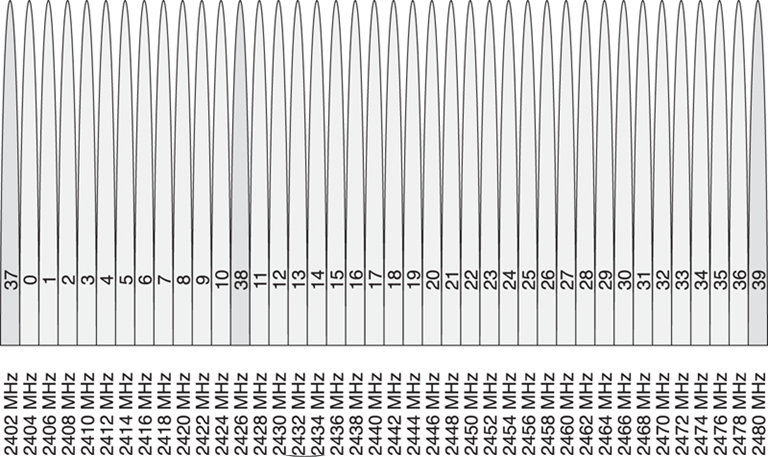
\includegraphics[width = 0.7\textwidth]{blechannels}
	\end{center}
	\caption{\ac{BLE} channels (advertisement channels render darker)}
	\label{fig:blechannels}
\end{figure}

\begin{figure}[htb]
	\begin{center}
		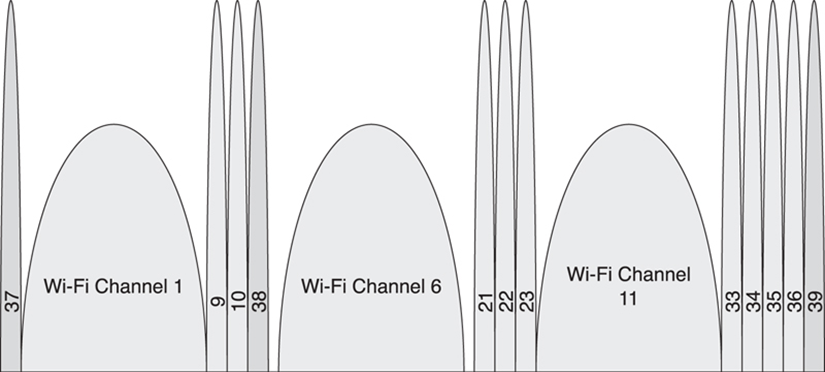
\includegraphics[width = 0.7\textwidth]{blechannelswifi}
	\end{center}
	\caption{\ac{BLE} channels with WiFi channels overlaid}
	\label{fig:blechannelswifi}
\end{figure}


The number of channels dedicated to advertising has also decreased, meaing less time is spent searching for discoverable devices. The advertisement channels have been specifically chosen not to interfere with the common WiFi channels. Finally, the radio characteristics are very dependent on temperature. Complex mechanisms are used to compensate and recalibrate on-the-fly radio parameters. Due to the episodic nature of \ac{BLE} the radio does not come under such thermal extremes. All these design changes have positive hardware ramifications. The reduced compelxity of \ac{BLE} means reduced hardware requirements (notably memory), in turn reducing the leakage current. 

\ac{BTC} was designed with the idea that it would be used to do many common jobs, and hence particular configurations were built into it. In \ac{BTC}, these configurations are known as profiles. Example profiles include the audio distribution profile (A2DP), which is used in by many Bluetooth product manufacturers to allow a device, such as a phone to interact with an audio system, such as in a car. Another example would be the serial port profile (SPP), meant to emulate the highly popular and robust RS-232 serial standard for data transfer (recall that \ac{BTC} was concieved as a solution to wires). This is all built into what is known as the Bluetooth stack – a software framework that interacts between the physical layer and the application layer\footnote{Depending on what level of the stack one is working, master can take the names central or client, while slave can take peripheral or server.}.  

\ac{BLE} also makes use of this paradigm but is often superficially depicted as \ac{BTC} operating at lower speeds and power consumption. It is not currently compatible with \ac{BTC} and there are no plans for it to be. Like \ac{BTC}, the \ac{BLE} architecture has 3 over-arching parts: Application, Host and Controller. The controller, simply put, is the radio and related hardware controllers and the application the use case, which could be a cadence monitor, thermometer or even an electroencephalogram. It is the host controller interface (HCI), commonly known as the “stack” that provides the necessary software to enable the application layer to communicate with the radio (see Figure~\ref{fig:ble_arch}).

\begin{figure}[htb]
	\begin{center}
		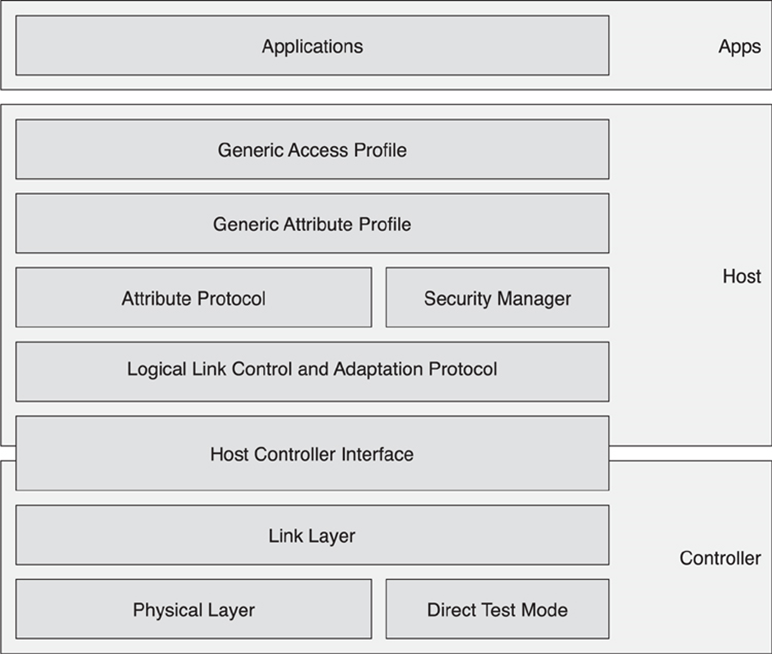
\includegraphics[width = 0.7\textwidth]{ble_arch}
	\end{center}
	\caption{\ac{BLE} Architecture}
	\label{fig:ble_arch}
\end{figure}

In an attempt to be economical with time and space components of the stack deemed irrelevant will not be discussed further here. For example a description of the security manager is not relevant as this project is not concerned with sending data over encrypted links. Similarly, the Logical Link Control and Adaption Protocol, while used extenivesly in all radio communication will not be discussed in detail as it doesn't provide any insight into maximising throughput or minimising power.

In \ac{BTC} profiles were diverse and large enough to warrant chip designers releasing tailored chips to perform well for a specific profile, i.e. a chip supporting A2DP may contain \ac{CODEC} hardware for real time audio streaming. In \ac{BLE} the profile framework is far lighter. \ac{BLE}'s profiles are all built ontop of  the \ac{GATT}, which in turn is built upon the \ac{ATT}, a protocol optimised to run on BLE devices. Attributes are an umbrella term, being the atomic unit of data communicated between BLE devices. Profiles are hierarchical constructions of attributes, in the top down order of profile, service, characteristic and descriptors, as shown in Figure~\ref{fig:exampleprofile}. A BLE device implements atleast one profile, \ac{GAP} along one more which is typically the purpose of the device. \ac{GAP} contains important information such the the device name and prefered connection properties.  This second profile can be one of the standard profiles as defined by the SIG group or a bespoke profile for the application, such as the case for a \ac{EEG}. Popular, SIG defined examples of \ac{BLE} profiles include the heart rate profile (HRP), health thermometer profile (HTP) and even a glucose profile (GLP) with room for many more to be incorporated into the core \ac{BLE} \ac{SIG} defined \ac{GATT} specifications.  

\begin{figure}[htb]
	\begin{center}
		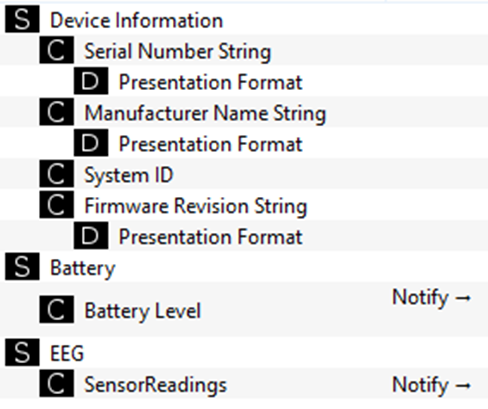
\includegraphics[width = 0.5\textwidth]{exampleprofile}
	\end{center}
	\caption{Example GATT profile consisting of 12 attribute - 3 services, 6 characteristics and 3 descriptors. }
	\label{fig:exampleprofile}
\end{figure}

 Attributes represent information about state. In the case of the greenhouse, the state would include the measured temperature. A suitable profile name which encapsulates the state is ''thermometer'', which contains the services ''device information'', ''battery service'', and ''thermometer''. As in figure~\ref{fig:exampleprofile}, the greenhouse thermometer service may contain the same device information and battery services, but replace the ''EEG'' service with the thermometer service, and the ''SensorReadings'' service with temperature. The other profile, \ac{GAP}, will contain the attributes which define how \ac{BLE} unit discover and establish connection to one another.  This includes the device name, perhaps ''greenhouse thermometer'', along with the preferred slave connection properties, e.g. a connection interval of 4 seconds, with a slave latency of 150 (10 minute window). All this information is contained within the GATT database, and shared as needed to other \ac{BLE} units. 

When communicating attributes, there are four data operations available. Read and write typically require one device to access the others characteristic. In the case of the greenhouse, the house device would request to read the thermometer. Notification and indications differ to read and write, in that the device(s) after information subscribes to the changes of state of the characteristics. For example, when greenhouse slave device wakes up, if the thermometer measurement changed, it will send a notification or indication alert the master device inside the house. The former methods can be thought of as synchronous means of communication while the latter asynchronous. Notifications differ from indications in that indications require a application level acknowledgment. That is, the indication is bubbled up to the user code, which then either accepts or rejects the indications. Notifications are acknowledge near the bottom of the \ac{BLE} stack, verifying correct receipt and message integrity. Therefore notifications are suitable for higher throughput applications. As shown in figure~\ref{fig:exampleprofile} shows notifications are operation configured for battery and EEG sensor readings. In this example, whenever the battery level changes, any devices subscribed to the characteristic battery level will receive a notification.

In \ac{BTC} the network topology used pico-nets, whereby one device has one master, but could be a master of another device. \ac{BLE} operates a simpler network topology, star, whereby a device can either be a master or slave, but not both. The master has the responsibility of organising itself between the slaves. If one slave requires large amounts of bandwidth, it my impact the quality of service encountered by the other devices. 

\begin{figure}[htb]
	\begin{center}
		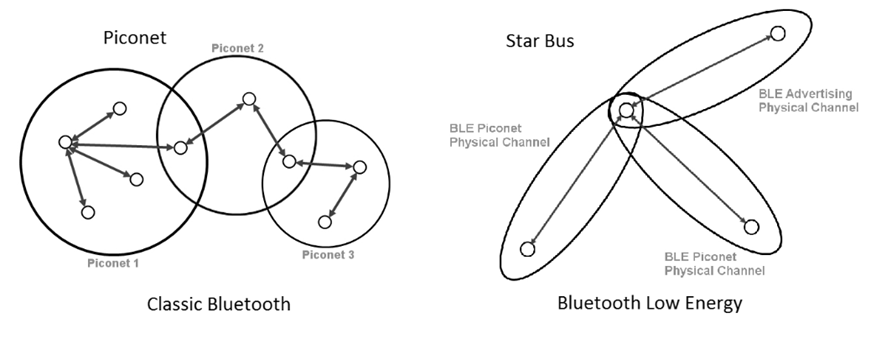
\includegraphics[width = \textwidth]{topology}
	\end{center}
	\caption{Bluetooth Network Topologies }
	\label{fig:topology}
\end{figure}

Both BLE and BTC devices move through generic system states. The same abstract view can be applied to both technologies and is shown in. Note that depending on the role of the device, the state moves right (master) or left (slave) from standby. It may appearing confusing to have another state for scanning which can only move into the standby state, but this is useful for searching and discovering devices with no commitment to connecting. Such a use case might be suitable for devices that intermittently broadcast small amounts of information. Assuming that the master BLE device is in the initiating state, searching for a connectable device, and at the same time the BLE slave is in the advertising stage, periodically broadcasting information using advertisement packets; the two devices will find one another and may initiate a connection request.

\begin{figure}[h]
	\begin{center}
		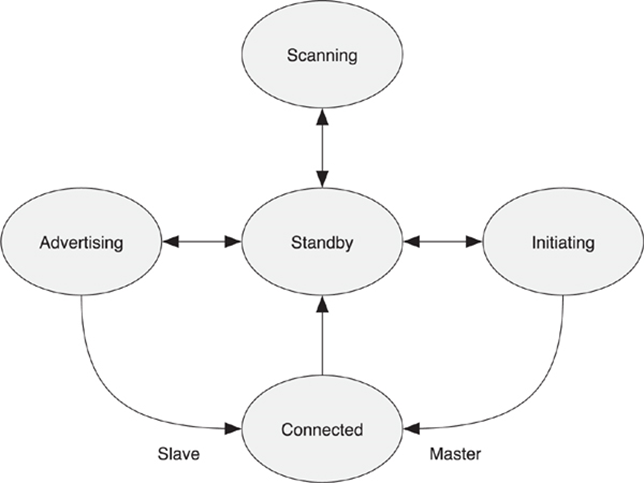
\includegraphics[width = 0.8\textwidth]{systemstate}
	\end{center}
	\caption{Device State Transition Diagram}
	\label{fig:systemstate}
\end{figure}

\ac{BLE} is principally composed of two types of packets, advertisement (Figure~\ref{fig:advertisement}) and data (Figure~\ref{fig:data}). Both packet types vary in length dependent on the payload but share a 32 bit advertising access address field, a 24 bit \ac{CRC} field, an 8 bit header and an 8 bit length field which defines the \ac{PDU} size (the last 2 field are often collectively called the header field). Advertisement \ac{PDU}s range from 0 to 29 bytes (232bits), meaning the total packet size can vary between 72 and 320 bits. The over-the-air data rate is 1Mbit/s, meaning advertisement packets are transmitted at a rate between 72 and 320$\mu$s (a single bit is transmitted every 1$\mu$s). In addition to the access code and \ac{CRC} fields, data packets consists of an 8 bit preamble and a \ac{PDU} varying between 0 and 27 bytes (4 of these bytes are reserved for encryption). Hence, the packet length varies from 80bits to 328 bits. 

\begin{figure}[!h]
	\centering
	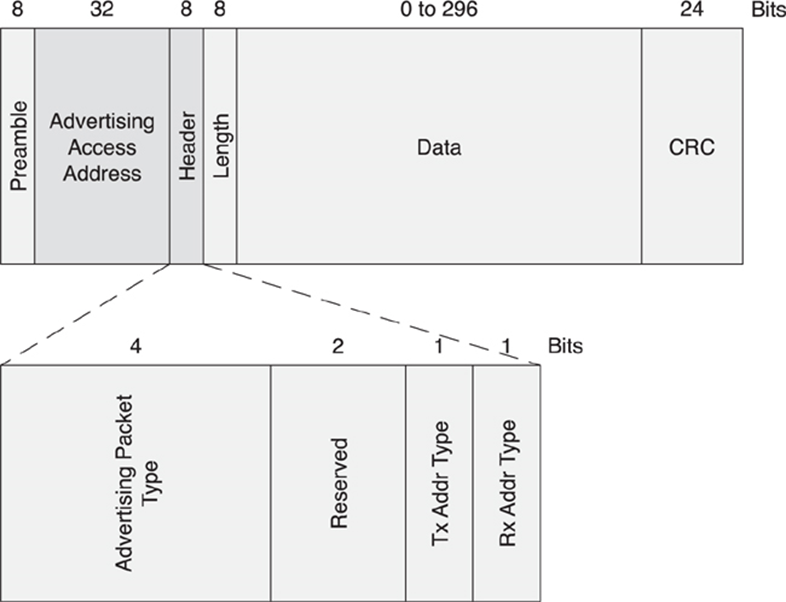
\includegraphics[width = 0.7\textwidth]{advertisement}
	\caption{\ac{BLE} Advertisement packet}
	\label{fig:advertisement}
	{Img advertisment}
\end{figure}

\begin{figure}[!h]
	\begin{center}
		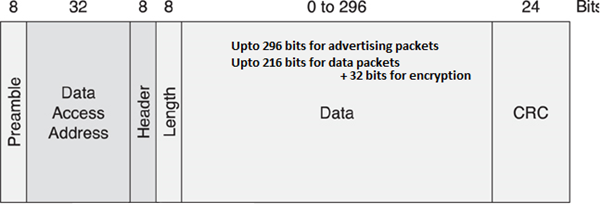
\includegraphics[width = 1\textwidth]{data}
	\end{center}
	\caption{\ac{BLE} Data packet}
	\label{fig:data}
\end{figure}

Figure~\ref{fig:connection} shows a connection between two devices being initiated. The first packet shown is is an indirect advertisement packet, available to all listening \ac{BLE} devices. The second packet is a connection request from the master device, communicating in the payload its address, the address to establish a connection with, and random access address, a connection interval length, the hop sequence, channel map, the connection timetout, slave latency and other things. Here the advertisement packets are rendered in green, the data in (predominantly) yellow (the magenta also represent a type of data packet)
\begin{itemize}

 \item The channel map bit pattern corresponds to a contiguous stream of 37 ones, corresponding to all 37 channels being operational (the master has no reason to prevent transmission). 
 \item The hop byte indicates between each \ac{CI} how many channels the device pair will increment. From packet 242 onwards, the channel map increments every \ac{CI} (2 packets/30ms).
 \item The access address is a randomly chosen number (by the master) which acts as a identifier for a connection between two devices. 
 \item The interval of 0x18 (24 decimal) represents the \ac{CI} length in units of 1.25ms. Therefore 0x18 represents 30ms between connection intervals. Between each master to slave directional data packet (every 2 packets), the total sum of the time is 30000$\mu$s

\end{itemize}

It is highlighted that (at least initally) the slave interval is 0, meaning the slave should wake up every \ac{CI}. In packets numbers 243 and 244, the slave and master respectively have nothing to send, and simply acknowledge on another with an empty \ac{PDU}. The protocol realises flow control through the the lazy acknowledgment of \ac{SN} and \ac{NESN} bits, embedded into the header of every data channel.

\begin{figure}[!h]
	\begin{center}
		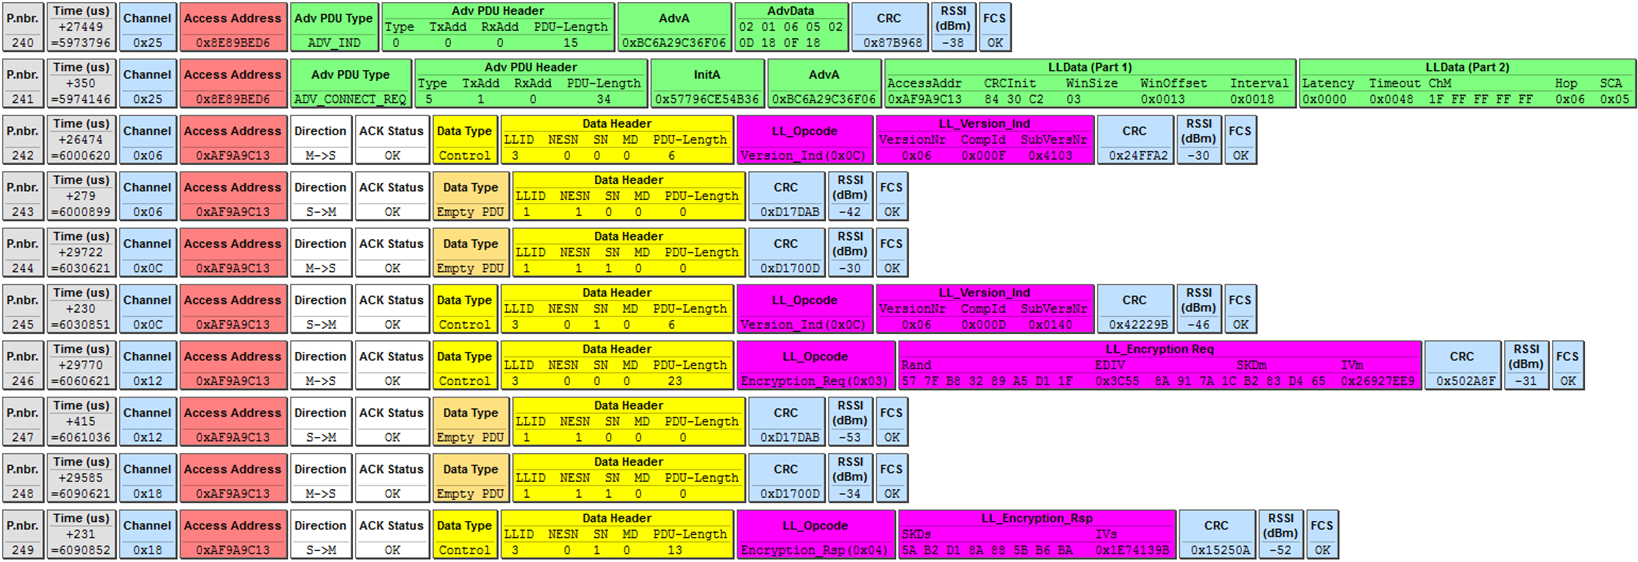
\includegraphics[width = 1.4\textwidth, angle=90]{connection}
	\end{center}
	\caption{\ac{BLE} connection initialisation}
	\label{fig:connection}
\end{figure}

While explained for completeness, advertisement and packets used in the initial establishment of a connection are of no concern to this project since they do not contribute to data throughput and once a connection has been established, do not contribute to the power consumption of the device. Hence, their contribution is removed from measurements as it is assumed the long term amortised cost is zero. The (incomplete) connection initialisation process shown in Figure~\ref{fig:connection} is known as "Just Works" pairing.



As previously mentioned, to achieve high throughputs notifications are used. To achieve the maximum throughput, it is desirable to send notifications as fast as possible. However, data cannot be sent out without flow control, and all notification packets must first be received then acknowledged before the next packet is sent. When a packet is sent, there is a mandatory 150$\mu$s inter-frame period. For the maximum throughput the connection receiving device would just acknowledge the data in an 80 bit acknowledgment response. Another 150$\mu$s frame would occur between this responding device and a transmitting device, bringing the total time up to:

\begin{displaymath}
328\mu s + 150\mu s + 80\mu s + 150\mu s = 708\mu s
\end{displaymath}

 This is shown graphically in Figure~\ref{fig:turnaround}. The total duty cycle is 

\begin{displaymath}
\frac{328\mu s}{708\mu s} \approx 58\%
\end{displaymath}
which is relatively low when compared radio technology duty cycles, e.g. \ac{BTC}. The 150$\mu$s inter frame period exists to prevents the silicon from heating to excessively, preventing power consuming hardware being required to recalibrate the radio. 

From the figure it is possible to calculate the upper bound for the number of packets that can be transmitted per second is

\begin{displaymath}\frac{1000000\mu s}{708\mu s} \approx  1414.43\;packetes/second\end{displaymath}

Of the 41 bytes (328 bits) sent for a notification packet, only 27 of them are considered for application use, and 4 of those are used for encryption. Even if encryption is not used, for complexity reasons, the maximum amount of application data is restricted 23 bytes.

\begin{displaymath}
1414.1293 \frac{packets}{s} \times 184 bits \approx 260 kbp/s
\end{displaymath}

While a lot of literate quote{CITATION PLEASE] this as the maximum usable data rate of this 23 bytes 3 bytes are required to identify the command type (notification) through an op-code (1 bytes) and which attribute it belongs to through an attribute handle (2 bytes). This means that only 20 bytes of the original 27 reserved for the application are usable, reducing the upper bound for throughput to 

\begin{displaymath}
1414.1293 \frac{packets}{s} \times 160 bits \approx 226 kbp/s
\end{displaymath}

Here forth, the usable payload of a "notification" or "data packet" is 20 bytes. When aiming for either low power and/or high efficiency, it is important fill the usable payload with as much data as possible, as every notification packet sent has a fixed cost of 80 bits associated with it. TALK ABOUT PCK EFFICIENCY 

\begin{figure}[h]
	centering
		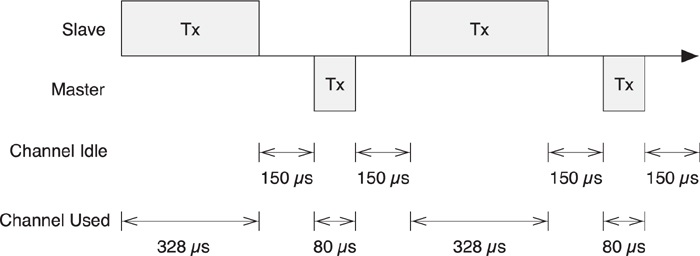
\includegraphics[width = 1\textwidth]{turnaround}
	\caption{\ac{BLE}'s packet flow for maximum throughput}
	\label{fig:turnaround}
\end{figure}

The \ac{BLE} specification defines no maximum 

The \ac{BLE} protocol was not designed for high throughput applications, but rather for low latency episodic communication devices transferring small data payloads of representing device state. The energy per bit is low compared other popular technologies, and should not be used as the bottom-line metric for performance. Rather, a holistic metric of the whole system energy consumption for a specific use case will form the basis of the performance metric in this report.

\clearpage

\section{Preliminary Research}

This section deals with evaluating the technology and radios
Equipment used to evaluate 

Wireshark etc

\subsection{Radio Evaluation}

There are a number of competing companies int the \ac{BLE} consume space. The most popular chip manufacturers at the time of evaluation are\ac{TI}, \ac{NS} and \ac{CSR}, although  other manufacturers exist, they normally design combo-wireless technology chips, e.g. Broadcomm, which only offers WiFi, \ac{BTC} and \ac{BLE} combined \ac{SoC}. These chips are not suitable for this project due to their complexity, packaging and intend application - the typical use case of such combo-chips are in high powered devices such as tablets, smart phones and notebooks. 

Different sources [citation] will calculate the application throughput differently. 

\ac{BLE} data packets can carry a payload of upto 20 bytes

After sourcing

%%%%%%%%%%%%%%%%%%%%%%%%%%
%%%%%%%%%%%%%%%%%%%%%%%%%%

\subsubsection{nRF8001}
The first radio tested was \ac{NS}'s nRF8001, selected due to the data sheet claiming it was the lowest power consuming device. The reason for this was because the chip only contained a controller and host layer. The application layer must be provided by an external micro controller, which is a large amount of effort to write. Fortunately a hobbyist open source project\cite{Guan2013} was available that provided the necessary code to get limited connectivity up and running. Figure~\ref{figure:nrf8001} shows the prototyping setup used to measure the performance of the nrf8001 microchip. 

Using a shunt resistor, the measured peak current was approximately 14.5mA, which correlates with the figure found in the data sheet (14.6mA). This was at a 

The ATMega328 consumes approximately XmA, however for the remainder. As the device was hardware limited to only 1 packet per connection event further development was abandoned.

\begin{figure}[h]
	\begin{center}
		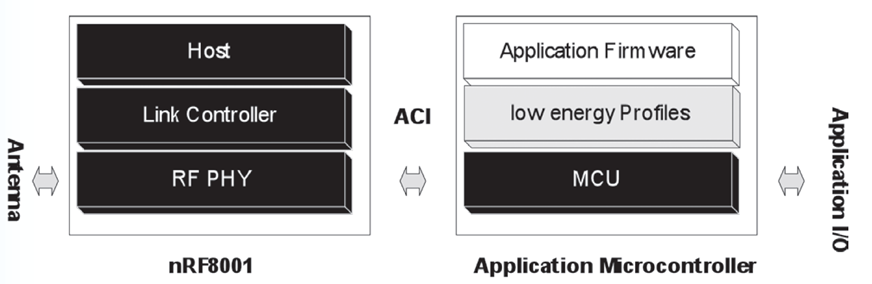
\includegraphics[width = 0.9\textwidth]{nrf8001stack}
	\end{center}
	\caption{nRF8001 application block diagram }
	\label{fig:nrf8001stack}
\end{figure}


\begin{figure}[H]
	\begin{center}
		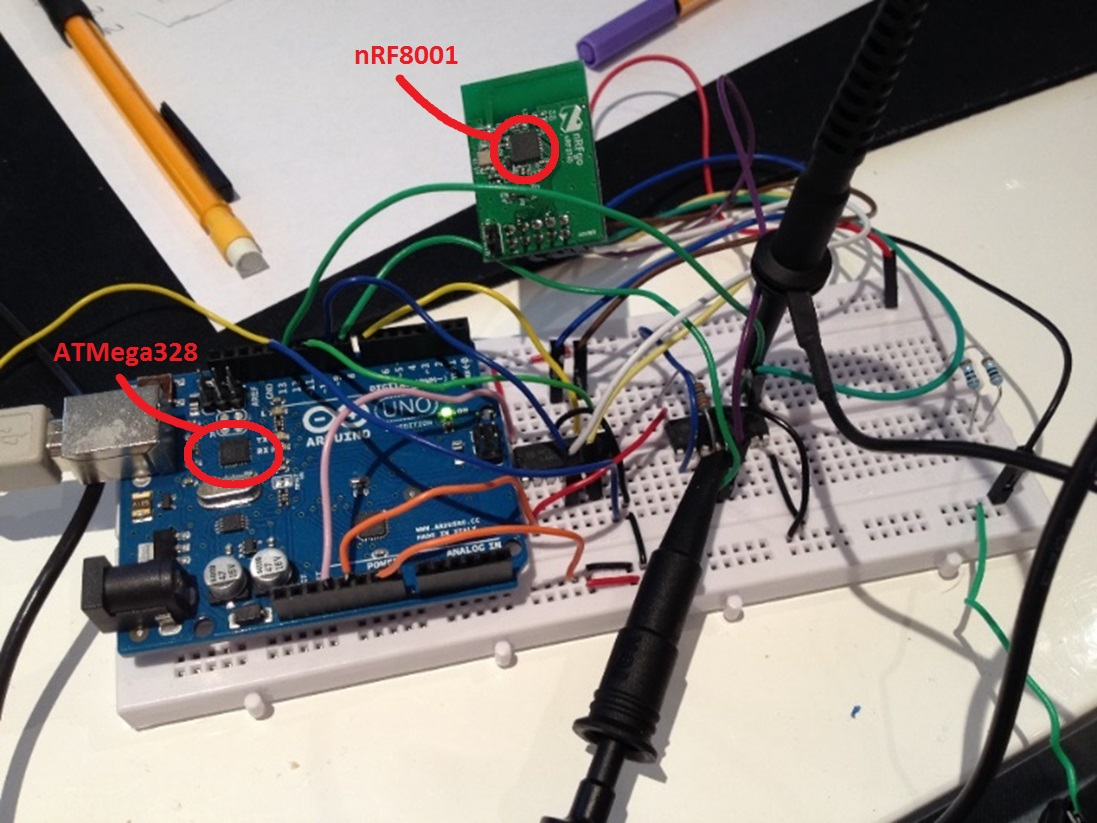
\includegraphics[width = 0.9\textwidth]{nrf8001}
	\end{center}
	\caption{Arduino Uno development board acting hosting the application layer for the nRF8001 radio. Level shifters were required for interfacing with the low-paper chip}
	\label{fig:nrf8001}
\end{figure}

\begin{figure}[H]
	\begin{center}
		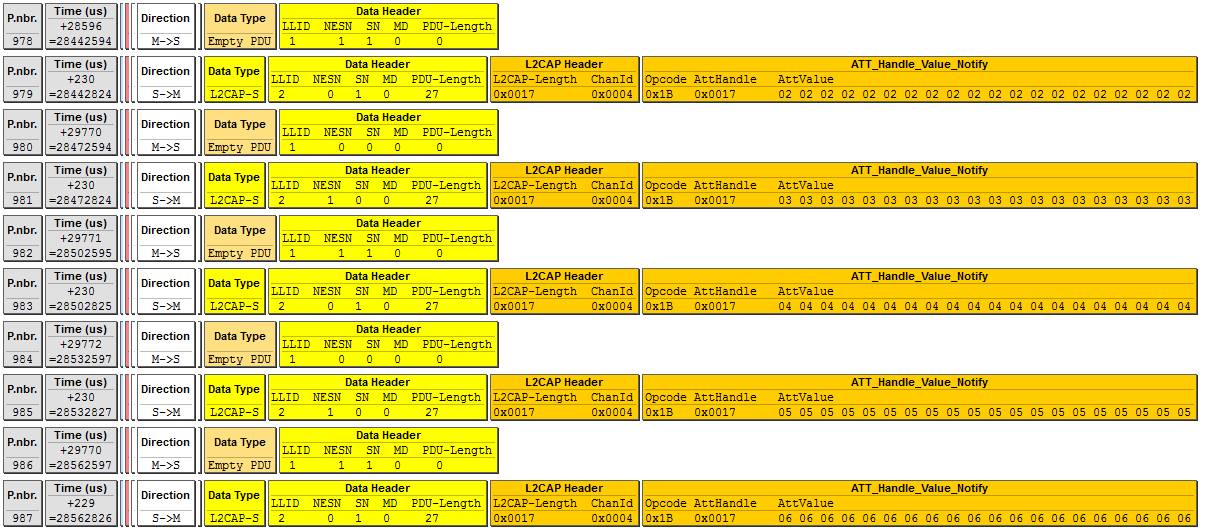
\includegraphics[width = 1.4\textwidth, angle=90]{nrfcap}
	\end{center}
	\caption{Packet-sniffed connection between Apple iPhone 4s and nrf8001. Notification rate 1 packet every 30ms. Some fields removed due to page space constraints}
	\label{fig:nrfcap}
\end{figure}

Initially, the device was configured to send a large amount of notification within a single \{CE} and at the lowest \ac{CI}. The master device was an Apple iPhone 4S, and it was found the total throughput was 5328 bit/s or 2.3% of the theoretical upper bound. The reason for such a low throughput was two fold. Apple restricts the minimum connection interval to 30ms through software (causing the slave \ac{CI} to increase. [CITE] It has been reported this is due to issues with their design, whereby many radio technologies share the same antenna. 30ms is four times greater than the minimum \ac{CI} available, hence this reduces the maximum throughput to 25% of theoretical maximum. The second reason, unlisted from the data sheet\cite{nrf8001}, is that the device is capable of only transmitting, on average, one packet per \ac{CE}. This is simply due to the hardware design, and ultimately believed to be why the device claims the lowest power out of all the radios. Figure~\ref{nrfcap} shows a packet capture



As the device can only send 1 packet per \ac{CI}, to achieve the highest throughput, the device must be run at the smallest connection interval of 7.5ms. At this interval the upper bound for throughput becomes

\begin{displaymath}
\frac{1000}{7.5} \times 20\:bytes \approx 2666\;byte/s
\end{displaymath}

With 16 channels at an 8 bit resolution, the highest frequency measurable (according to Nyquist condition) is 

\begin{displaymath}
\frac{1 2666\; byte/s}{16} \times \frac{1}{2} \approx 83  Hz
\end{displaymath}

A maximum support frequency running a solo channel is approximately 1328 Hz.

\subsubsection{nRF51822}
Another \ac{NS} product tested was the nRF51822. Information on the suppport packets per connection event was also not present in the datasheet\cite{nrf51822}. This device was found capable of receiving up to 6 packets per second, and this was verified by an engineer\cite{olme}. While a marked improvement over the nRF8001, this meant that the device was only capable of operating at 60% of the maximum throughput capable as claimed in the specification. The maximum support frequency per channel for 16 channels at 8 bits resolution is 500Hz.

Unfortunately the chip came as part of a larger development kit and accurate power measurements were not attainable, however the support softwares suite included a power calculator [CITE BATTERY SECTION].

\subsubsection{CSR1010}
Through direct contact with \ac{CSR} engineers, it was reported a particular single mode \ac{BLE} radio device, CSR1010, was capable of reaching the full throughput as defined in the \ac{BLE} specification. \ac{CSR} supplied a development kit and software suite. The CSR1010 is part of \ac{CSR} 's new $\mu$Energy product line, for which \ac{CSR} have developed their own compiler and \ac{IDE} known as xIDE. 

For initial throughput testing, an example health thermometer application was used. \ac{CSR} provided a \ac{USB} dongle reported capable of 

From exploring and understanding the main features of the \ac{OSAL}, it was possible to increase the number of notification packets sent per connection interval from 1 to 8. Unfortunately, it was   

The standard mechanism provided for radio communication, is for every connection interval, receive successful confirmation of the first acknowledge.  This mechanism provides visibility at the \ac{CE} level, but not at the notification packet level - if many notifications are sent and acknowledged, this method doesn't provide any information that the \ac{CE} may have room for more notifications. This is a problem when large throughputs are desired, as the buffer queue is 8 packets in size. When more than 8 are added to the queue Hence, through the naive method, whereby notifications are placed into the queue before or after the start of the \ac{CE}, upto a maximum of 8 notifications are possible. This mechanism is visualised in Figure~\ref{fig:nols}. 

\begin{figure}[H]
	\begin{center}
		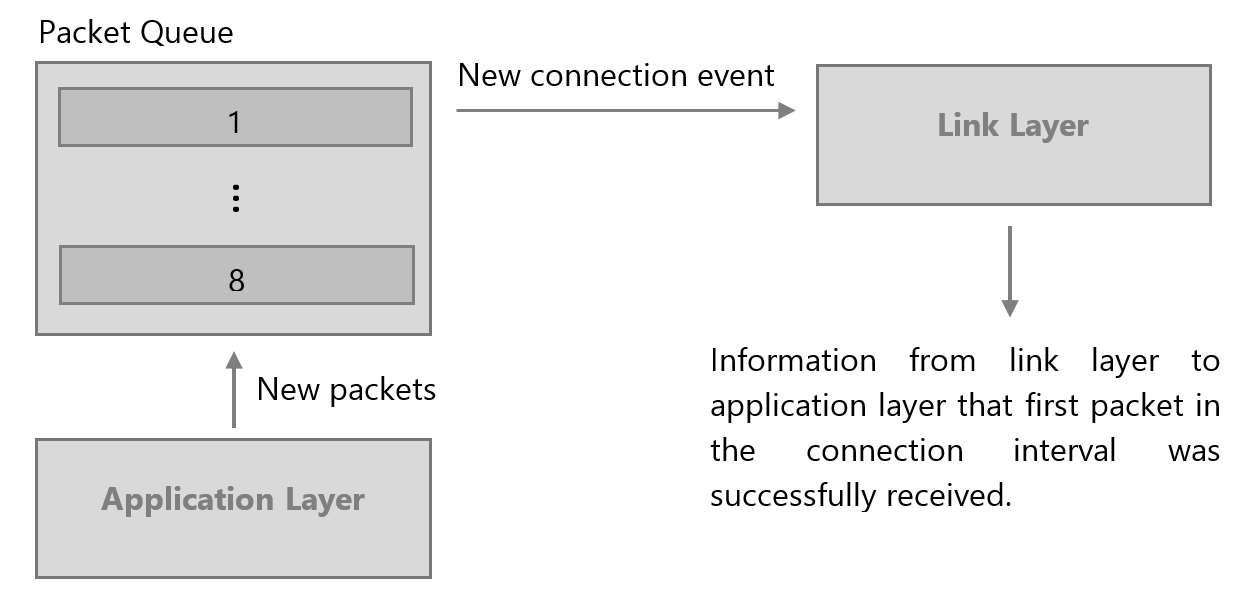
\includegraphics[width = \textwidth]{nols}
	\end{center}
	\caption{Notification of the first packet}
	\label{fig:nols}
\end{figure}

An experiment to test throughput was setup whereby each connection event sends 8 notifications per connection event with the same payload, bar one byte which increments with the connection event. The output can be seen in Figure~\ref{fig:8pckt}.

\begin{figure}[H]
	\begin{center}
		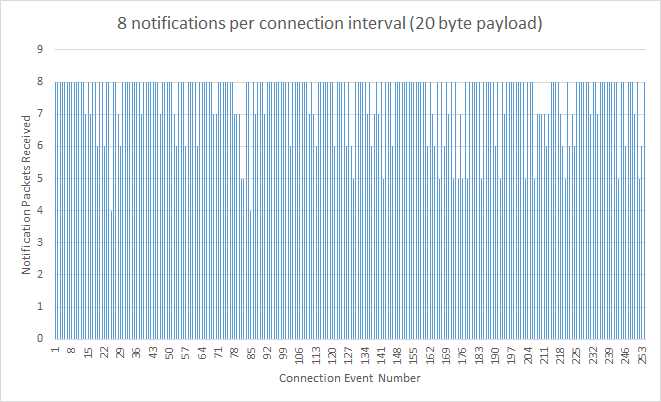
\includegraphics[width = 0.8\textwidth]{8pckt}
	\end{center}
	\caption{Queuing of 8 packets being lost}
	\label{fig:8pckt}
\end{figure}

From the experiment above, the conclusion was that the link layer stack became flooded with notification requests. Had the requests been accepted into the stack, then they would of been transmitted. If they failed to arrive at their destination, then the flow would of caused a negative acknowledgment, and the packet would of been retransmitted. Provided the notification made it through the link layer stack, it should appear in the output. 

After greater exploration of the software system framework, the \ac{API} and software mechanisms, it's possible use the message pump to signal whenever a packet is acknowledged. Upon receiving this signal, the device can then dispatch a subsequent packet. Figure~\ref{fig:lsrad} shows such a mechanism. 

\begin{figure}[!h]
	\begin{center}
		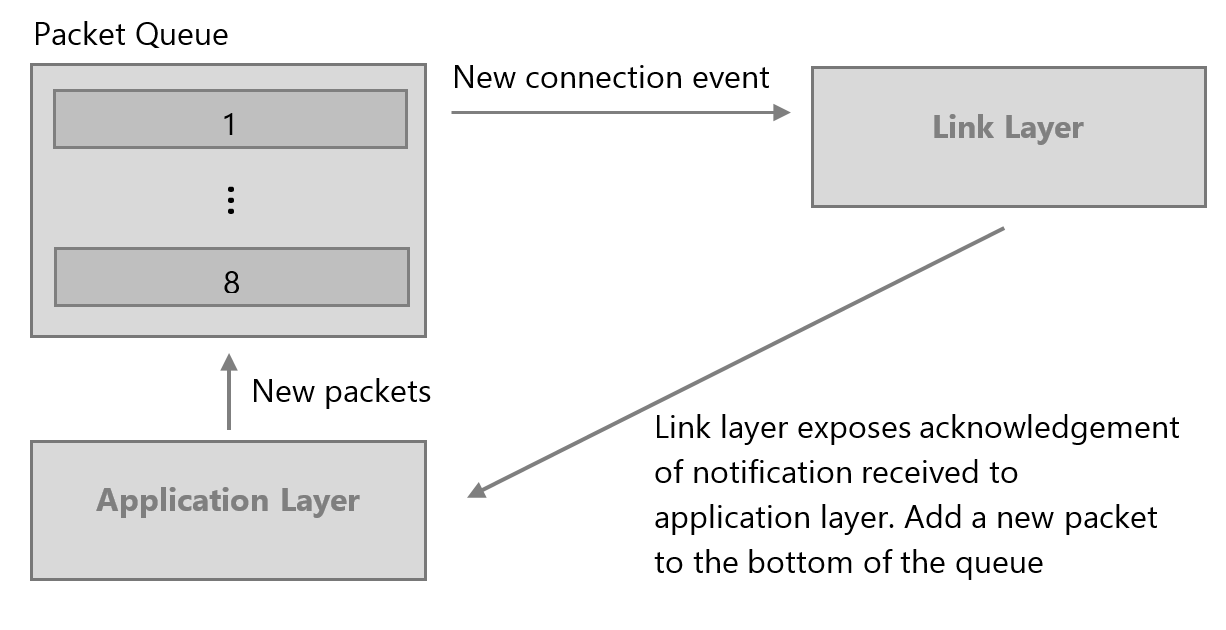
\includegraphics[width = \textwidth]{lsrad}
	\end{center}
	\caption{Upon packet acknowledgment }
	\label{fig:lsrad}
\end{figure}

The experiment was repeated again, this time sending a new notification every time the previous one was acknowledged. The results are shown in Figure~\ref{fig:9pckt}

\begin{figure}[!h]
	\begin{center}
		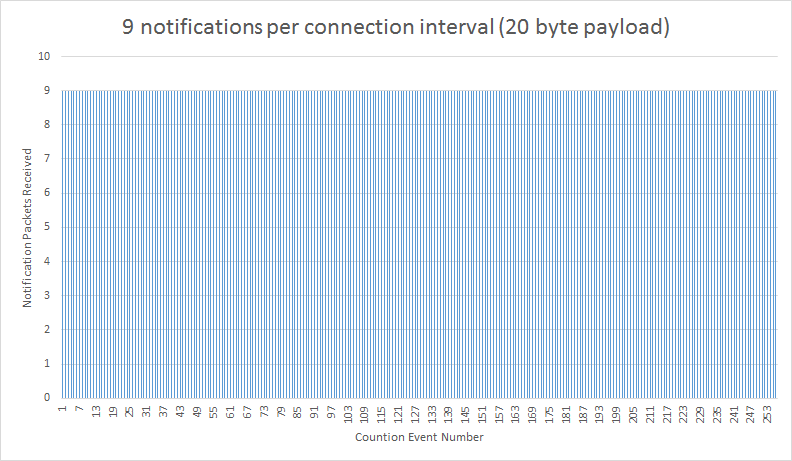
\includegraphics[width = \textwidth]{9pckt}
	\end{center}
	\caption{9 packets being received per connection interval when through acknowledgment feedback mechanism}
	\label{fig:9pckt}
\end{figure}
 
A capture of the notification data was taken over a period of approximately 46 seconds. Figure~\ref{fig:wireshark} shows part of the capture. 

\begin{figure}[h]
	\begin{center}
		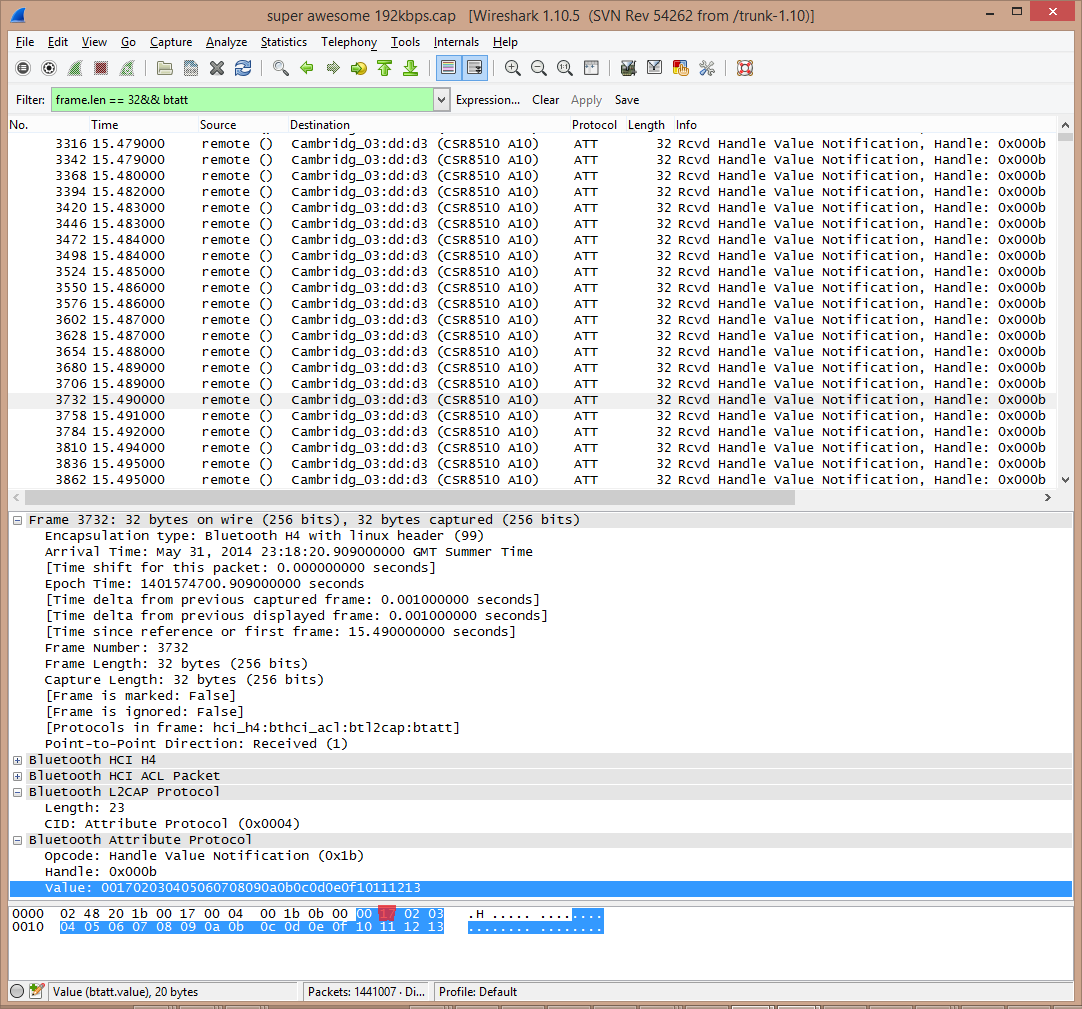
\includegraphics[width = \textwidth]{wireshark}
	\end{center}
	\caption{Packet capture. 20 byte data payload (blue) and connection event counter variable highlighted (red)}
	\label{fig:wireshark}
\end{figure}

In the 46.060 second period a total of 55286 notification packets were captured, bringing the average throughput to


\begin{displaymath}
\frac{55286}{46.060} = 1200.30395137\; packets/s
\end{displaymath}

For a 7.5ms \ac{CI}, the number of \ac{CE} is 133.333 and the number of packets per connection interval is

\begin{displaymath}
\frac{1200.30395137}{133.3333} = 9.0027\; packets/s
\end{displaymath}



A comprehensive explanation of the code is provided in the later section \ref{Prototype}. 

Initially the 



\subsubsection{CC2540 and CC2541}
\ac{TI}'s CC2541 is part of the sensor tag package - a \ac{BLE} one of the first, and arguably the most popular [need to CITE?] development kits. The CC2540 differs in that it's range and power usage are increased, though it's throughput is still theoretically the same.

Again, the associated white papers did not document the packet throughput per connection event. Through contact with a \ac{TI} employee [CITE], there is a hardware limitation of 4 buffers, limiting only 4 packets per connection event (each buffer contains 1 packet). Each buffer is 128 bytes in length, while \ac{BLE} data packets can be a maximum of 41 bytes. Through using an exposed firmware (software) switch it was possible to increase the throughput slightly to achieve 5 packets per connection event by refilling the buffers within the connection event, once the packet has been link layer acknowledged. Again, this was discovered through a Texas instrument employee. This increased the average packets per connection event to approximately 4.6, bringing the total throughput between 10-12.3k byte/s.

The CC2541 (and also CC2540) is a full \ac{SoC} - a programmable \ac{MCU} is packages togeter with the radio hardware. This has certain economical advantages, as common hardware and footprint is shared between the radio and \ac{MCU}. However, the Nordic company Chipcon who originally developed the hardware (Texas Instruments has since acquired them), relied on the Swedish tool chain provider, IAR, for the development tool suite and chain. \ac{TI} still relies up this tool software suite, haven't not invested in their own facilities to develop for the platform. A single software license is approximately 2000 USD. While IAR do offer a code-limited version, it is too small to contain all the necessary libraries. IAR also provide a 30 day trail, which is what is currently being used for evaluation, but proceeding with this chip for the prototype may be economically impossible.

Much like the CSR1010, a similar \ac{OSAL} existed for the CC2540/1, 

For 16 channels running simultaneously, at 8 bit resolution, the highest achievable detectable frequency is approximately 384 Hz.


\subsection{Batteries}
There are many different battery technologies available. For the device a small, low profile low footprint, lightweight battery is required. Given that BLE can consume up to 15mA of peak current, taking this as the upper bound means that for 12 hours of continuous use batteries with capacities of 180mAh should be considered. Although the radio will dominate, other parts of the circuit such as the Microprocessor will consume a small amount of power, so this figure is arbitrarily upped to 200mAh. Note that peak current is an unfair way to measure current consumption in BLE, however it is being used here as a worst case scenario. 

Two batteries technologies which satisfy this technology are Lithium Ion (the popular CR2032 or other) or Zinc-air batteries with capacities of 600mAh cheaply available. Common voltages are 1.4V to 1.65V (radios require between 1.8 -3.6V). However the batteries are so light, less than 2g each (one CR2032 weighs, on average, over 3g), they can be combined in series to provide a suitable voltage and a large capacity (over 1Ah). Further, this high voltage will allow the effective radio range of the BLE device to increase. If a Zinc cell exhibits damage, unlike most technologies, no dangerous chemicals are present. The downside to zinc-air batteries is that they must be vented to an oxygen environment (cannot be hermetically sealed) which in turn causes them to lose their charge over time relatively quick once exposed to air. Although \ac{EEG} use case requirements will require the device to lifetime of hours to days, not years. 

Two Zinc-air batteries weighing 1.9g each, can supply over 1000mAh with a combined series voltage of 2.8V. In the worst case of BLE drawing 15mA, this will last almost 3 days. Recall 15mA is the peak current and BLE will never continuously draw this current, hence the lifetime of the device should be greater. BLE was designed that current is never continuously consumed, and between radio events, the battery has recovery periods, extending the useful life of the battery (Heydon, 2012). 

Nordic semiconductor provides a studio which has a battery lifetime calculator. Using a typical lithium ion battery of 220mAh yields, 7.5ms connection interval and 100% connection, yields a lifetime of ~163hours. This makes sense as the current average current consumption is slightly above 1.3mA and the capacity of the battery is 220mA. If it is assumed that the number of packets sent scales linearly, we can divide this number by 4 to obtain a throughput of 10.4 Kbytes and a lifetime of 40 hours (Figure 21). It cannot be verified how accurate this model is, but the simulation looks sensible. Figure 22 shows a notification simulation of the EEG service being sent continuously every 7.5ms. Notice the peak current is the transmit current followed immediately by a receive current (waiting for the link layer acknowledgement from the master). Dividing by 4 may overestimate the actual power consumption is the integral over the whole time, not just the small Tx peak, which is comparable to the start-up, Rx and processing currents (Figure 14 & Figure 22).
 

\begin{figure}[htb]
	\begin{center}
		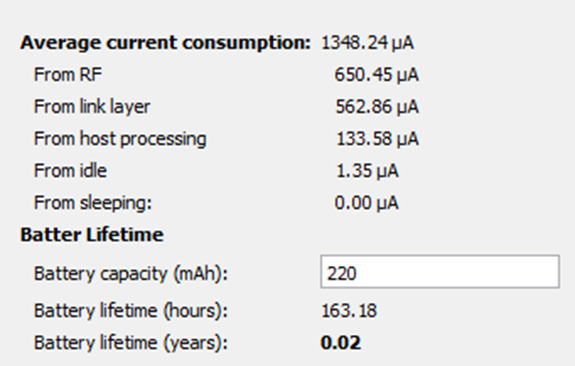
\includegraphics[width = 0.5\textwidth]{nrfsim}
	\end{center}
	\caption{Power consumption and lifetime calculator}
	\label{fig:nrfsim}
\end{figure}

\begin{figure}[htb]
	\begin{center}
		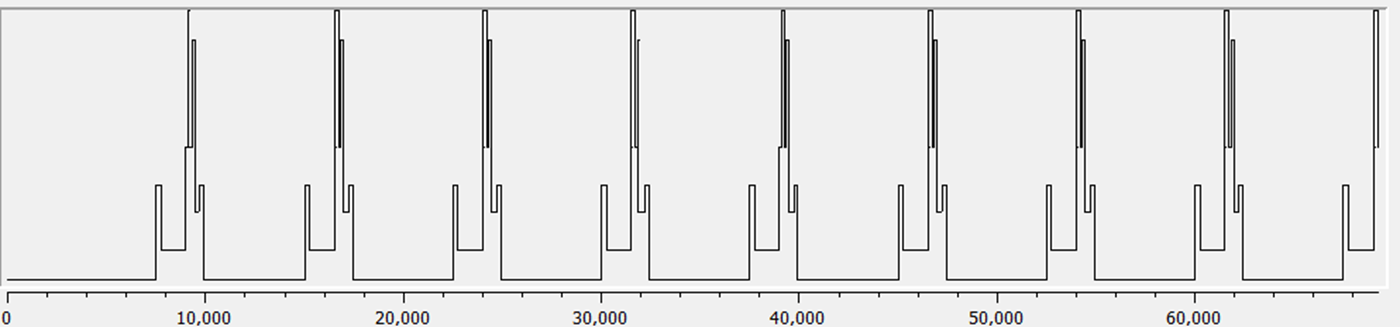
\includegraphics[width = 1.1\textwidth]{nrfwave}
	\end{center}
	\caption{nRF8001 waveform (1 transmission per connection event}
	\label{fig:nrfwave}
\end{figure}

 
Figure 23 - Simulation plot of notifications being sent
For 2 zinc-air batteries of 500mAh capacities, this model predicts the device lifetime under nominal operation begins to reach 10 days.  An intelligent estimate to how this module is generated is linked to the throughputs calculated at the start of the Radios section. As each bit represents 1 micro second it is very easy to integrate for set parameters the time over time the current profiles to achieve an estimate of power usage. 
Max drain current is another important concept to consider. Batteries can only safely deliver a maximum amount of current. If the battery is stressed to deliver more current that it is rated, it will degrade the overall lifetime of the battery. 

\subsection{Microcontroller}
There are a couple of options here. Often radios are provided as a system on chip (SoC), whereby the microchip contains not just the radio but also a fully functional microcontroller unit (MCU). Often these devices will consume more power than just the host and controller, but the system as a whole will typically consume more power overall if the application is run on an off chip MCU. 
 
Figure 15 - SoC (a) and a typical 2 chip solution (b) (Heydon, 2012)
It really comes down to the application, as having the application on an off-chip MCU may mean that power is saved overall as other features such as ADCs, SPI interfaces and other peripherals can be utilised and integrated into the application without having to run a separate application on both the external MCU and radio chip, which leads to increased overhead, complexity and power. 

For development purposes the Arduino family of development boards, which sport many different processors seem like an excellent for development. These processors have many features such as GPIO, inbuilt ADCs, dedicated SPI pins, etc. Further, there is an extensive documentation, large knowledge base and a very active online forum. Of particular interest are the earlier Arduino models which utilise the very low power Atmel 8-bit family of processors. A further plus is that these processors are available in both DIP and SMT packages, meaning they are suitable breadboard prototyping. The ATMega328 seems like a particurly good choice, as a balance between support, power and simplicity. 

Currently, Texas Instrument’s SensorTag have been investigated along with Nordic semiconductors nRF8001. The former is a SoC solution while the latter only implements the host and controller layers. Implementing an application layer is no small feat, and fortunately it was possible to make contact with someone who has developed libraries to drive the chip using an Arduino microcontroller. Please see the section titled Experimentation and Current  for more information.

Currently the general feeling is towards using an Arduino microcontroller simply due to the ease and rapid nature of development. Some components (an particular ADC and the nRF8001) have been tested and confirmed to work with the device.


\subsection{Component Selection}

Apple CIs
Ti code studio
Android phones must support 4 packet/ CI
Ease of development
ADCs

While the CC2541 showed promise as with enough hardware understanding and firmware switches, it may mean the device could approach the theoretical limit, the unavailability of an inexpensive tool chain meant software development was problematic. The CSR1010 is supplied with a free tool chain and \ac{IDE}, as \ac{CSR} engineers confirmed experiments with the device operating with high throughputs. The package of the radios were both similar, being of roughly the same size \ac{QFN} package type, which while reported outside the department's \ac{PCB} production capabilities, was still considered of sufficiently large for in-house prototyping. 

Ultimately the final component selection for the \ac{EEG} prototype
\begin{itemize}
\item AD7997 ADC 
\item CSR1010
\item P675 Zinc Air batteries. Batteries of capacity 620mAh are readily available and inexpensive. Two are required in series to achieve correct voltage
\end{itemize}



\section{Specification}

\section{Prototype Design}

The first iteration of the board. Due to the process capabilities and materials used, the radio frequency traces were not impedance matched, and the device range was limited to approximately 7 meters within a building or 15 meters \ac{LOS}. 

\begin{figure}[htb]
	\begin{center}
		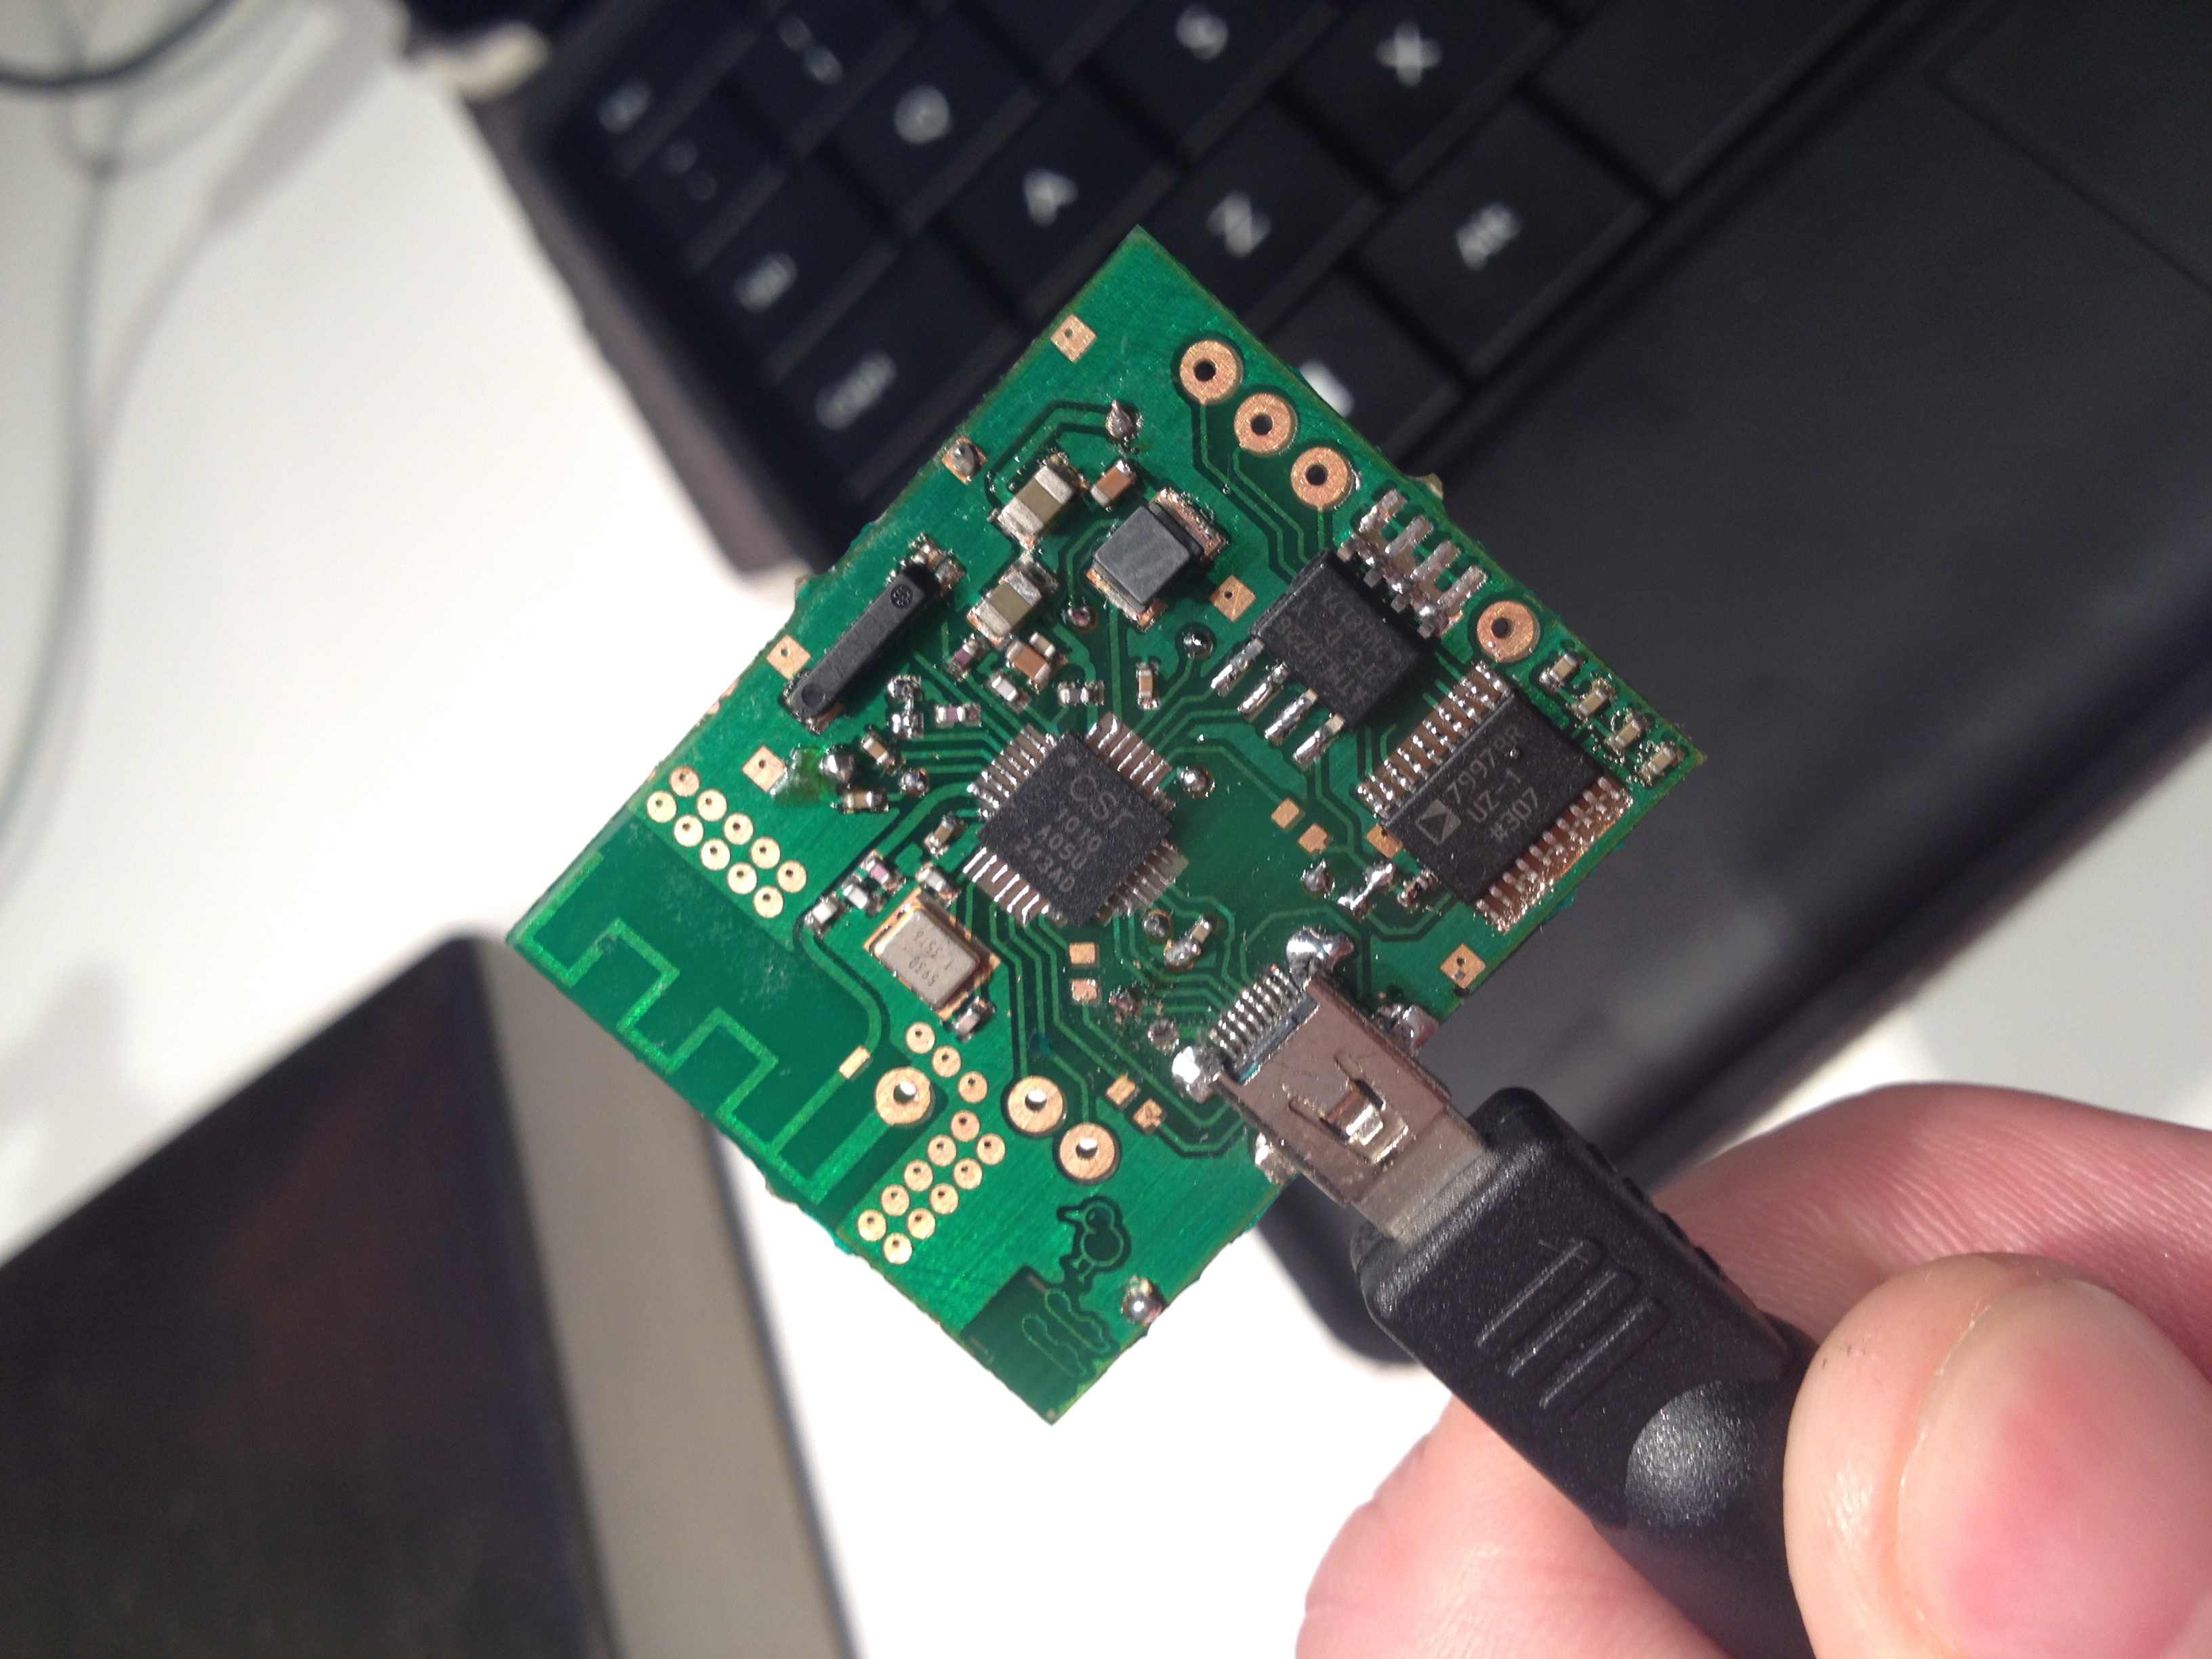
\includegraphics[width = 0.9\textwidth]{pcb1.jpg}
	\end{center}
	\caption{First PCB iteration}
	\label{fig:pcb1.jpg}
\end{figure}

\subsection{Component Selection}

\section{Results}

Weighing in at a total of 

\section{Evaluation}

\subsection{Power Analysis}

The hardware

Assuming that the number of 

The idea of minimising energy per bit is not the true picture, as \ac{BTC} and WiFi have higher energy per bit ratios. To achieve the lowest energy per bit, the transmission rate needs to be at the highest throughput achievable on the hardware due to the fixed costs or sunk costs of waking the \ac{MCU} and preparing the device for radio transmission. However, consistently running at such throughput invalidates the use case for \ac{BLE}, as there are other technologies capable of transmitting at the same or higher throughputs for smaller energy requirements.




\subsection{Bill of materials}



\clearpage 
\section{Conclusions and Future Work}
The majority of interesting \ac{EEG} signals exist between . Running an \ac{EEG} device at that 

The proposed device is comparable to a hearing aid, even using the same battery technology. 

In the sole pursuit of maximizing throughput, the idea is to 

\begin{displaymath}
\min_{x}  \frac{1250\times x}{708} - \floor{ \frac{1250\times x}{708}} 
\end{displaymath}

Mathematically this finds the points where 

Unfortunately a connection interval must be between 7.5ms and 4000ms long, in incremental steps of 1.25ms. Therefore x must exist in the range of 6 to 3200. 

//but unfortunately, there is an energy cost associated with hardware buffers from operation and leakage current

Hard to classify


On the whole, the project has 
Both ends of the link 

Not all tablets will be able to run at full speed

Ideally, it is desirable to write a conference style paper. 

Never list packets per CI

Useful for CSR, monies worth out of me

Duplex

\section{Final Remarks}
A vast array of technologies and tools were used throughout this project. Below highlights those that are non-trivial and were of significant importance

\begin{itemize}
	\item Git verisioning control - For versioning and segmenting the workflow
	\item xIDE - CSRs integrated development suite for compiling and debugging CSR-stack based chips. This is where the firmware for the CSR1010 MCU was written
	\item Wireshark - Invaluable in analysing the packets and control flow between BLE radios, unfortunately must be used offline
	\item SmartRF online packet sniffer - Useful as a low-speed packet sniffer. Extremely useful in the early days of the project, however the throughputs eventually obtained rendered the tool and hardware redundant as it was not capable of such speeds
	\item Visual Studio 2013 - Primairly used for developing the tablet application. Highly useful for "knocking up" quick throughput expirements 
\end{itemize}

The large amount of both written and generated code is to vast to warrant being included in this report. Therefore is has been decided to make it publically available online at the git repositry address 
\url{https://github.com/proftom/AmbulatoryEEG}.

\section{Bibliography}
\clearpage

\nocite{*}

\printbibliography


\section{Appendix}
\subsection{Acronyms}
\begin{acronym}
	\acro{EEG}{Electroencephalography}
	\acro{BLE}{Bluetooth Low Energy}
	\acro{BTC}{Bluetooth Classic}
	\acro{CSR}{Cambridge Silicon Radio}
	\acro{TI}{Texas Instruments}
	\acro{NS}{Nordic Semiconductor}
	\acro{GATT}{Generic Attribute Profile}
	\acro{GAP}{Generic Access Profile}
	\acro{ATT}{Attribute Protocol}
	\acro{CI}{connection interval}
	\acro{SIG}{Special Interests Group}
	\acro{CODEC}{coder/decoder}
	\acro{CRC}{Cyclic Redundancy Check}
	\acro{PDU}{Packet Data Unit}
	\acro{SN}{Sequenc Number}
	\acro{NESN}{Next Expected Sequence Number}
	\acro{LOS}{line of sight}
	\acro{SoC}{system on chip}
	\acro{MCU}{microcontroller}
	\acro{API}{application programming interface}
	\acro{IDE}{integrated development environment}
	\acro{OSAL}{operating system abstraction layer}
	\acro{USB}{Universal Serial Bus}
	\acro{PCB}{printed circuit board}
	\acro{QFN}{quad flat no-leads}
\end{acronym}

\section{User Guide}
\end{document}